% Indicate the main file. Must go at the beginning of the file.
% !TEX root = ../main.tex

%%%%%%%%%%%%%%%%%%%%%%%%%%%%%%%%%%%%%%%%%%%%%%%%%%%%%%%%%%%%%%%%%%%%%%%%%%%%%%%%
% 03_results
%%%%%%%%%%%%%%%%%%%%%%%%%%%%%%%%%%%%%%%%%%%%%%%%%%%%%%%%%%%%%%%%%%%%%%%%%%%%%%%%


\section{Results}
\label{section3}

\subsection{Performance of the best Model}%%%%%%%%%%%%%%%%%%%%%%%%%%%%%%%%%%%%%%

The best performing configuration for the model was found to be the one with the following hyperparameters:

\begin{itemize}
    \item \textbf{n\_mels:} 64
    \item \textbf{n\_res\_blocks:} 4
    \item \textbf{learning\_rate:} 0.001
    \item \textbf{kernel\_size:} 5
\end{itemize}

On the test set, the model achieved an accuracy of 0.649 and an F1 score of 0.546. 
The confusion matrix for the predictions generated by this model is shown in Figure \ref{fig:confusion_matrix_best}.
The concentration of results in the diagonal of the confusion matrix indicates that the model is performing well.
Class 22 was predicted the most frequent with more than 50\% of the predictions being wrong.

\begin{figure}[h!]
    \centering
    \captionsetup{width=.7\linewidth}
    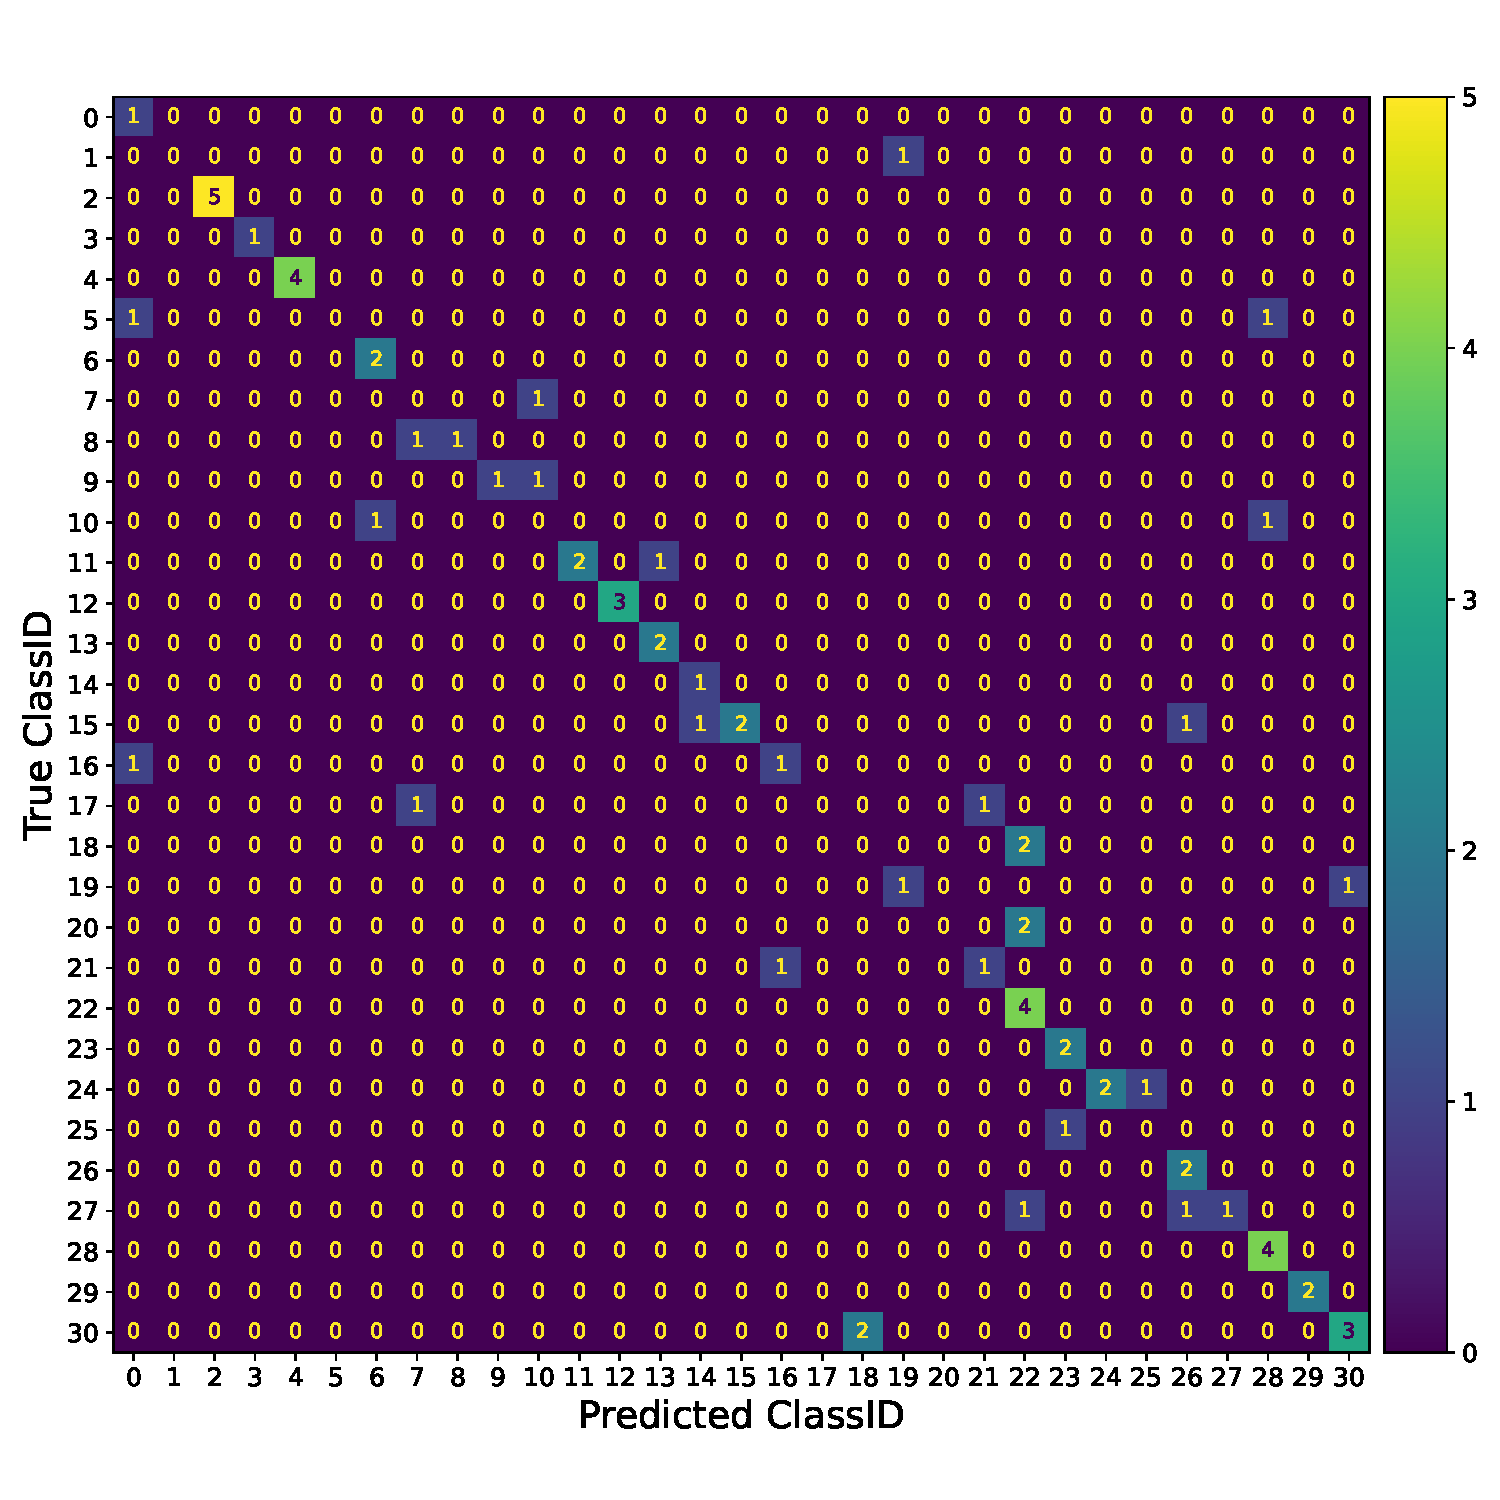
\includegraphics[width=1\textwidth]{figures/confusion_matrix_best.pdf}
    \caption{Confusion matrix for the predictions of the test set using the best model.}
    \label{fig:confusion_matrix_best}
\end{figure}

\subsection{Hyperparameter Tuning}%%%%%%%%%%%%%%%%%%%%%%%%%%%%%%%%%%%%%%%%%%%%%%

The detailed results of the Hyperparameter tuning are shown in table \ref{tab:hyperparameters_results}.

\begin{figure}[h!]
    \centering
    \captionsetup{width=.7\linewidth}
    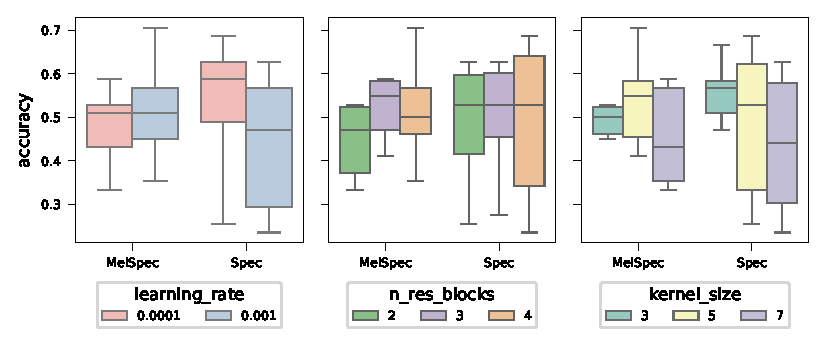
\includegraphics[width=1\textwidth]{figures/hyperparameters_boxplot.pdf}
    \caption{Accuracy of the models for different hyperparameter grouped by the transformation type.}
    \label{fig:hyperparameters_boxplot}
\end{figure}

\begin{figure}[h!]
    \centering
    \captionsetup{width=.7\linewidth}
    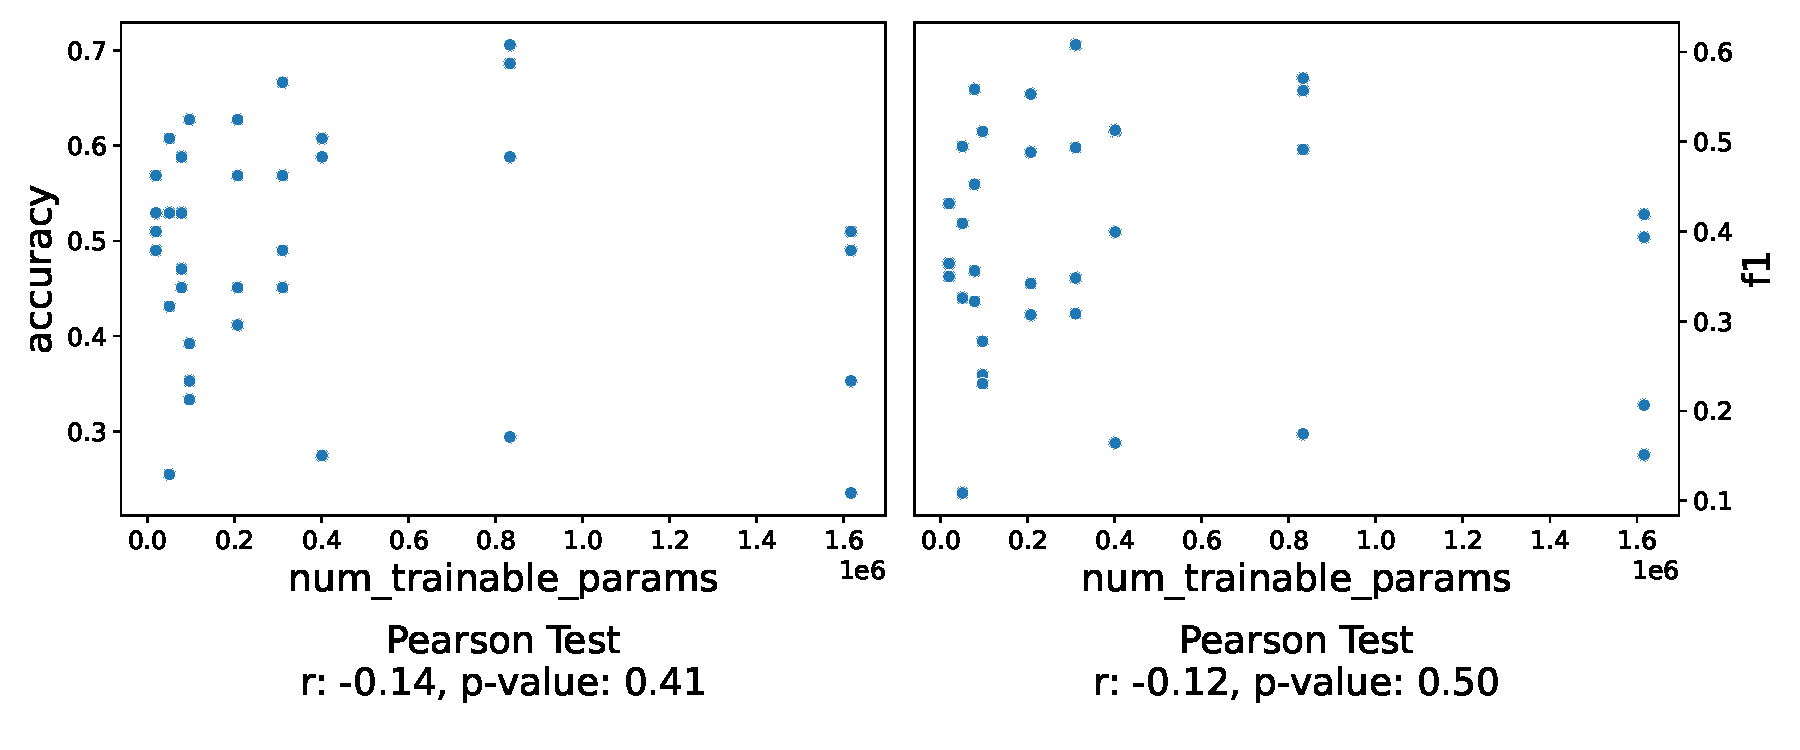
\includegraphics[width=1\textwidth]{figures/hyperparameters_scatterplot.pdf}
    \caption{Model size compared to the accuracy and F1 Score of the models.}
    \label{fig:hyperparameters_scatterplot}
\end{figure}

\begin{figure}[h!]
    \centering
    \captionsetup{width=.7\linewidth}
    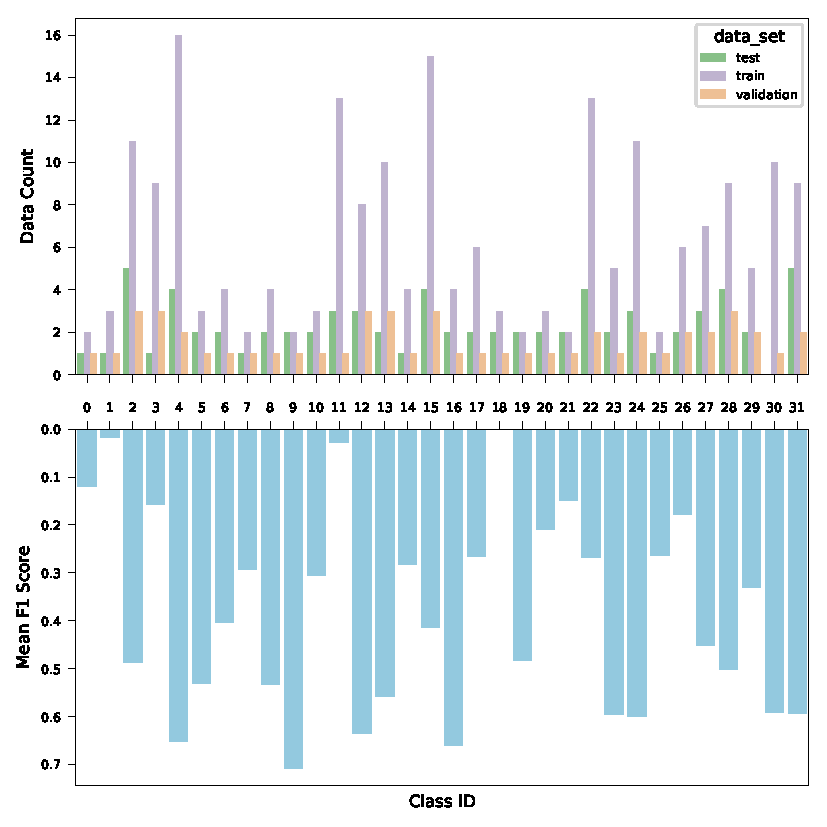
\includegraphics[width=1\textwidth]{figures/f1_per_class.pdf}
    \caption{F1 Score per class as mean trough all models compared to data distribution.}
    \label{fig:f1_per_class}
\end{figure}



